% Created by tikzDevice version 0.12.6 on 2024-05-22 14:39:46
% !TEX encoding = UTF-8 Unicode
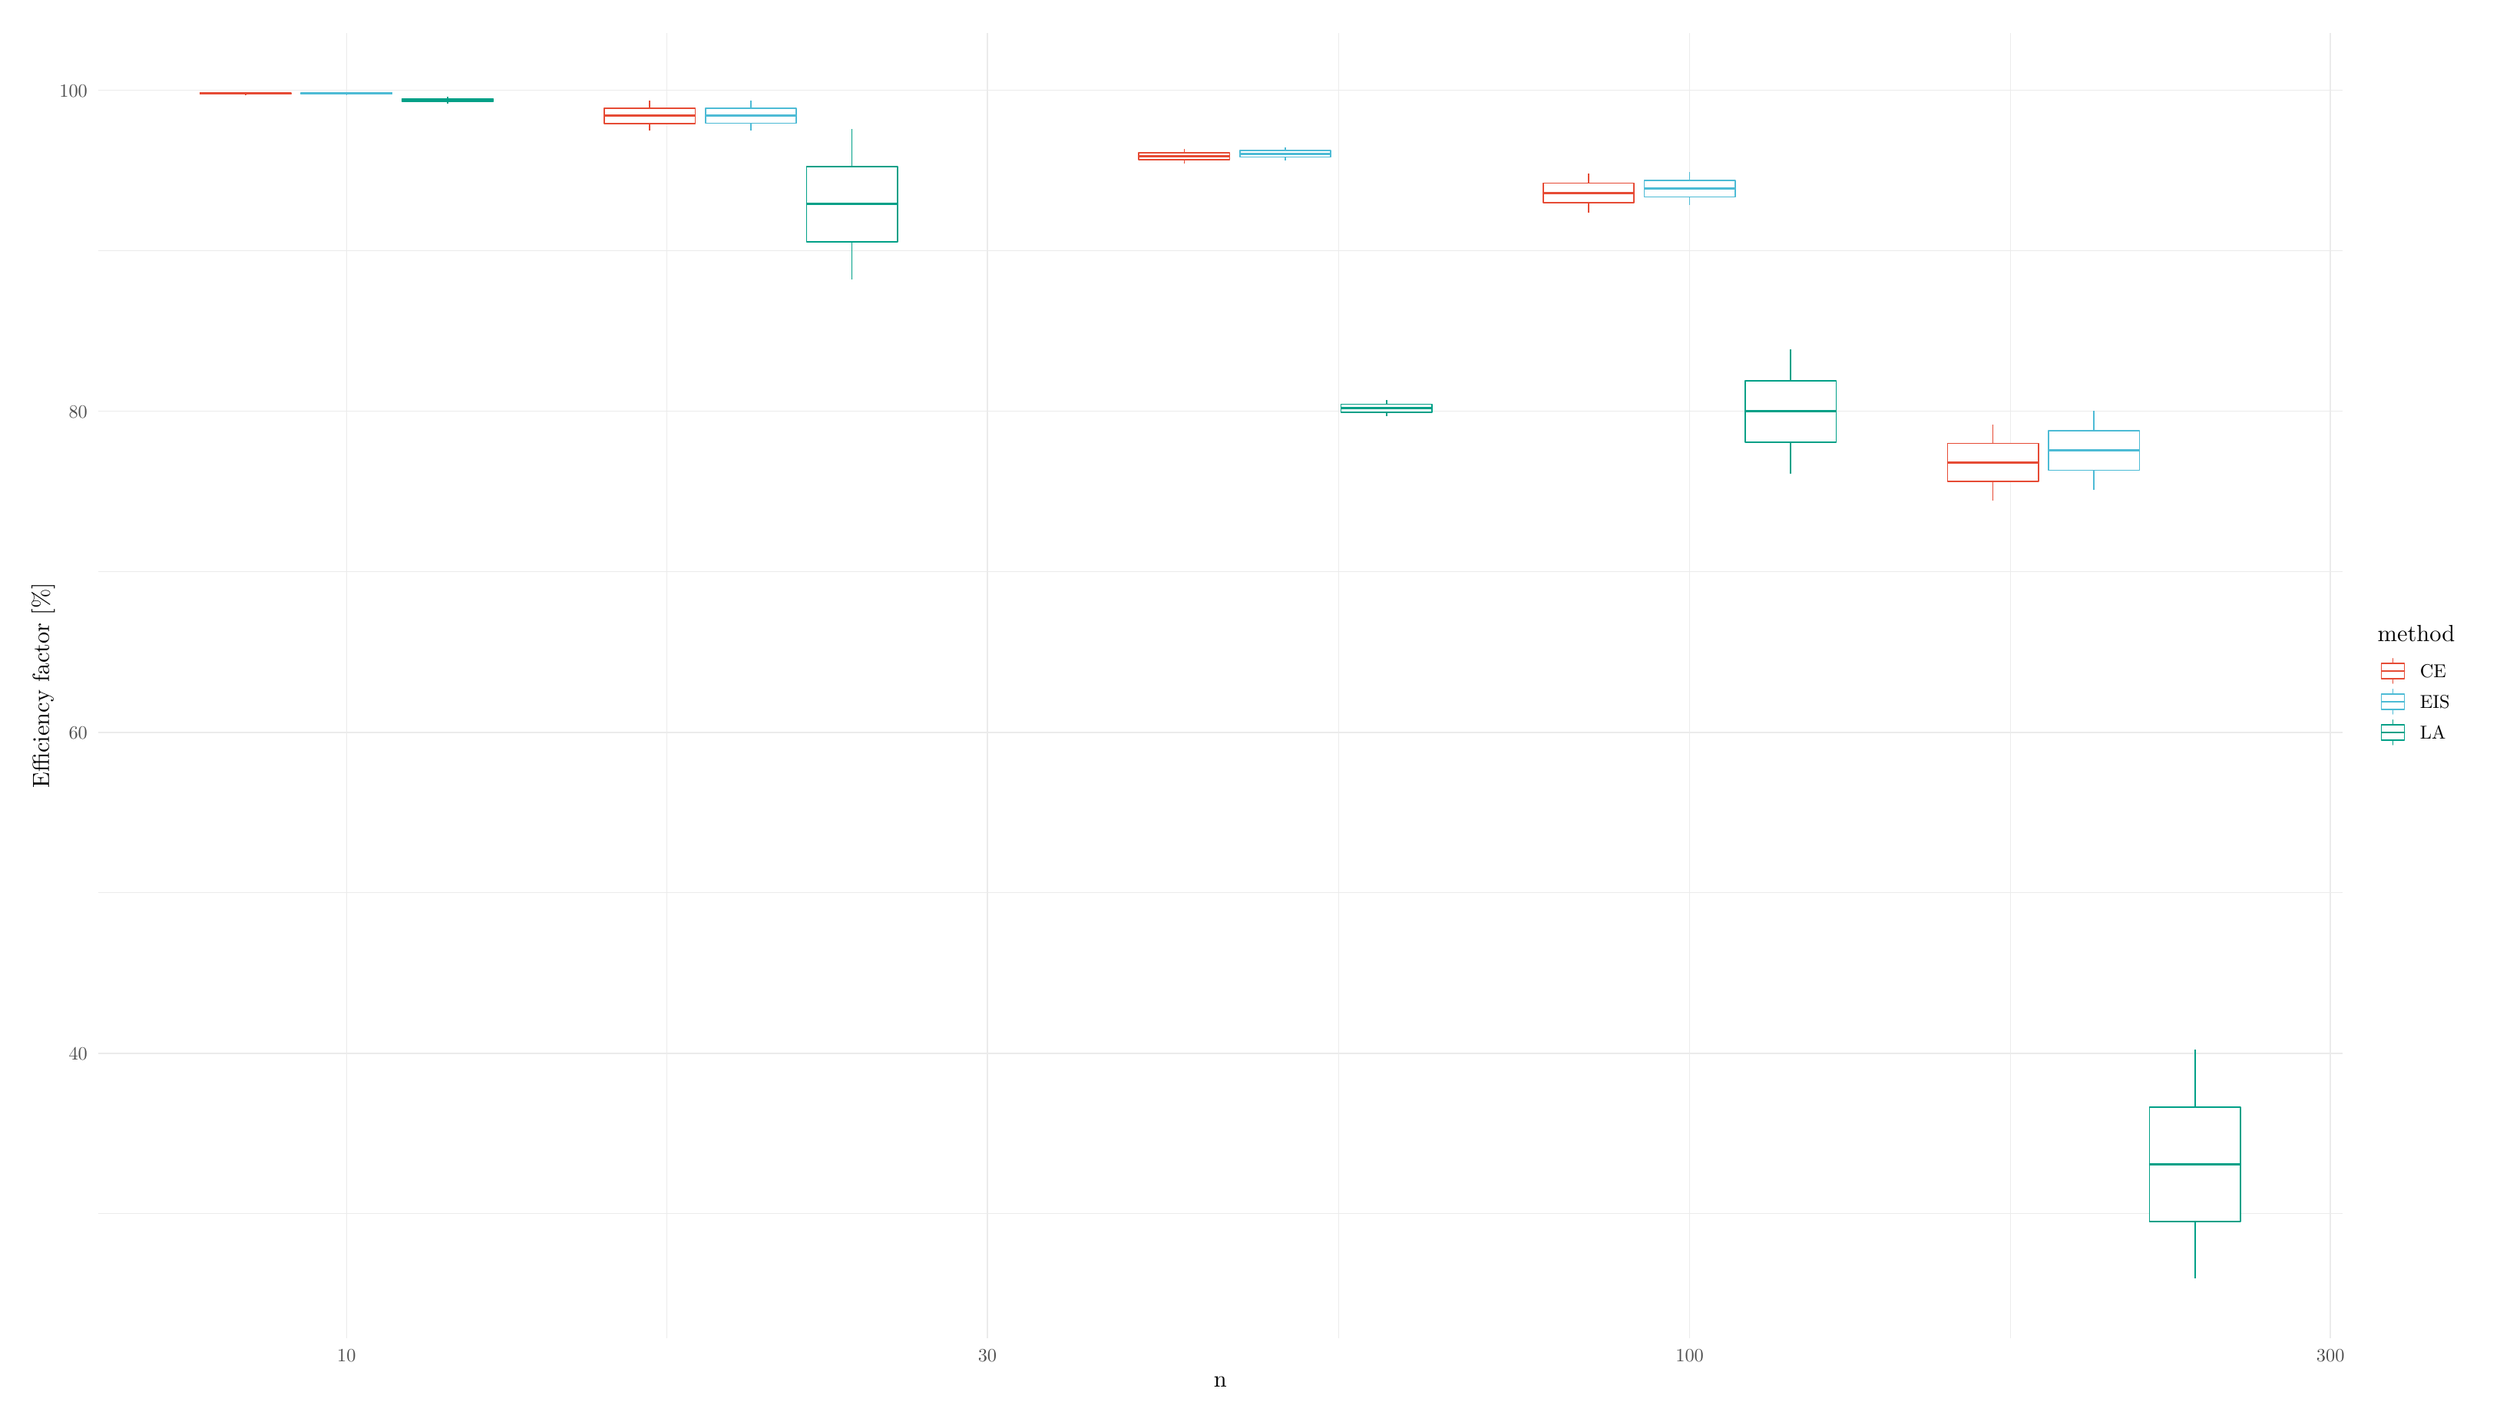
\begin{tikzpicture}[x=1pt,y=1pt]
\definecolor{fillColor}{RGB}{255,255,255}
\path[use as bounding box,fill=fillColor,fill opacity=0.00] (0,0) rectangle (1156.32,650.43);
\begin{scope}
\path[clip] ( 36.11, 30.69) rectangle (1092.47,644.93);
\definecolor{drawColor}{gray}{0.92}

\path[draw=drawColor,line width= 0.3pt,line join=round] ( 36.11, 89.19) --
	(1092.47, 89.19);

\path[draw=drawColor,line width= 0.3pt,line join=round] ( 36.11,240.26) --
	(1092.47,240.26);

\path[draw=drawColor,line width= 0.3pt,line join=round] ( 36.11,391.33) --
	(1092.47,391.33);

\path[draw=drawColor,line width= 0.3pt,line join=round] ( 36.11,542.40) --
	(1092.47,542.40);

\path[draw=drawColor,line width= 0.3pt,line join=round] (303.90, 30.69) --
	(303.90,644.93);

\path[draw=drawColor,line width= 0.3pt,line join=round] (619.94, 30.69) --
	(619.94,644.93);

\path[draw=drawColor,line width= 0.3pt,line join=round] (935.99, 30.69) --
	(935.99,644.93);

\path[draw=drawColor,line width= 0.6pt,line join=round] ( 36.11,164.72) --
	(1092.47,164.72);

\path[draw=drawColor,line width= 0.6pt,line join=round] ( 36.11,315.79) --
	(1092.47,315.79);

\path[draw=drawColor,line width= 0.6pt,line join=round] ( 36.11,466.86) --
	(1092.47,466.86);

\path[draw=drawColor,line width= 0.6pt,line join=round] ( 36.11,617.93) --
	(1092.47,617.93);

\path[draw=drawColor,line width= 0.6pt,line join=round] (153.10, 30.69) --
	(153.10,644.93);

\path[draw=drawColor,line width= 0.6pt,line join=round] (454.69, 30.69) --
	(454.69,644.93);

\path[draw=drawColor,line width= 0.6pt,line join=round] (785.20, 30.69) --
	(785.20,644.93);

\path[draw=drawColor,line width= 0.6pt,line join=round] (1086.78, 30.69) --
	(1086.78,644.93);
\definecolor{drawColor}{RGB}{230,75,53}

\path[draw=drawColor,line width= 0.6pt,line join=round] (105.53,616.69) -- (105.53,616.99);

\path[draw=drawColor,line width= 0.6pt,line join=round] (105.53,616.10) -- (105.53,615.80);
\definecolor{fillColor}{RGB}{255,255,255}

\path[draw=drawColor,line width= 0.6pt,line join=round,line cap=round,fill=fillColor] ( 84.13,616.69) --
	( 84.13,616.10) --
	(126.94,616.10) --
	(126.94,616.69) --
	( 84.13,616.69) --
	cycle;

\path[draw=drawColor,line width= 1.1pt,line join=round] ( 84.13,616.39) -- (126.94,616.39);

\path[draw=drawColor,line width= 0.6pt,line join=round] (295.81,609.43) -- (295.81,612.96);

\path[draw=drawColor,line width= 0.6pt,line join=round] (295.81,602.35) -- (295.81,598.82);

\path[draw=drawColor,line width= 0.6pt,line join=round,line cap=round,fill=fillColor] (274.41,609.43) --
	(274.41,602.35) --
	(317.22,602.35) --
	(317.22,609.43) --
	(274.41,609.43) --
	cycle;

\path[draw=drawColor,line width= 1.1pt,line join=round] (274.41,605.89) -- (317.22,605.89);

\path[draw=drawColor,line width= 0.6pt,line join=round] (547.35,588.56) -- (547.35,590.26);

\path[draw=drawColor,line width= 0.6pt,line join=round] (547.35,585.16) -- (547.35,583.46);

\path[draw=drawColor,line width= 0.6pt,line join=round,line cap=round,fill=fillColor] (525.94,588.56) --
	(525.94,585.16) --
	(568.75,585.16) --
	(568.75,588.56) --
	(525.94,588.56) --
	cycle;

\path[draw=drawColor,line width= 1.1pt,line join=round] (525.94,586.86) -- (568.75,586.86);

\path[draw=drawColor,line width= 0.6pt,line join=round] (737.63,574.25) -- (737.63,578.85);

\path[draw=drawColor,line width= 0.6pt,line join=round] (737.63,565.05) -- (737.63,560.45);

\path[draw=drawColor,line width= 0.6pt,line join=round,line cap=round,fill=fillColor] (716.22,574.25) --
	(716.22,565.05) --
	(759.03,565.05) --
	(759.03,574.25) --
	(716.22,574.25) --
	cycle;

\path[draw=drawColor,line width= 1.1pt,line join=round] (716.22,569.65) -- (759.03,569.65);

\path[draw=drawColor,line width= 0.6pt,line join=round] (927.91,451.78) -- (927.91,460.73);

\path[draw=drawColor,line width= 0.6pt,line join=round] (927.91,433.88) -- (927.91,424.94);

\path[draw=drawColor,line width= 0.6pt,line join=round,line cap=round,fill=fillColor] (906.50,451.78) --
	(906.50,433.88) --
	(949.31,433.88) --
	(949.31,451.78) --
	(906.50,451.78) --
	cycle;

\path[draw=drawColor,line width= 1.1pt,line join=round] (906.50,442.83) -- (949.31,442.83);
\definecolor{drawColor}{RGB}{77,187,213}

\path[draw=drawColor,line width= 0.6pt,line join=round] (153.10,616.72) -- (153.10,617.01);

\path[draw=drawColor,line width= 0.6pt,line join=round] (153.10,616.15) -- (153.10,615.86);

\path[draw=drawColor,line width= 0.6pt,line join=round,line cap=round,fill=fillColor] (131.70,616.72) --
	(131.70,616.15) --
	(174.51,616.15) --
	(174.51,616.72) --
	(131.70,616.72) --
	cycle;

\path[draw=drawColor,line width= 1.1pt,line join=round] (131.70,616.44) -- (174.51,616.44);

\path[draw=drawColor,line width= 0.6pt,line join=round] (343.38,609.50) -- (343.38,613.04);

\path[draw=drawColor,line width= 0.6pt,line join=round] (343.38,602.43) -- (343.38,598.90);

\path[draw=drawColor,line width= 0.6pt,line join=round,line cap=round,fill=fillColor] (321.98,609.50) --
	(321.98,602.43) --
	(364.79,602.43) --
	(364.79,609.50) --
	(321.98,609.50) --
	cycle;

\path[draw=drawColor,line width= 1.1pt,line join=round] (321.98,605.97) -- (364.79,605.97);

\path[draw=drawColor,line width= 0.6pt,line join=round] (594.92,589.52) -- (594.92,591.02);

\path[draw=drawColor,line width= 0.6pt,line join=round] (594.92,586.50) -- (594.92,584.99);

\path[draw=drawColor,line width= 0.6pt,line join=round,line cap=round,fill=fillColor] (573.51,589.52) --
	(573.51,586.50) --
	(616.32,586.50) --
	(616.32,589.52) --
	(573.51,589.52) --
	cycle;

\path[draw=drawColor,line width= 1.1pt,line join=round] (573.51,588.01) -- (616.32,588.01);

\path[draw=drawColor,line width= 0.6pt,line join=round] (785.20,575.56) -- (785.20,579.45);

\path[draw=drawColor,line width= 0.6pt,line join=round] (785.20,567.77) -- (785.20,563.88);

\path[draw=drawColor,line width= 0.6pt,line join=round,line cap=round,fill=fillColor] (763.79,575.56) --
	(763.79,567.77) --
	(806.60,567.77) --
	(806.60,575.56) --
	(763.79,575.56) --
	cycle;

\path[draw=drawColor,line width= 1.1pt,line join=round] (763.79,571.66) -- (806.60,571.66);

\path[draw=drawColor,line width= 0.6pt,line join=round] (975.48,457.70) -- (975.48,467.03);

\path[draw=drawColor,line width= 0.6pt,line join=round] (975.48,439.05) -- (975.48,429.72);

\path[draw=drawColor,line width= 0.6pt,line join=round,line cap=round,fill=fillColor] (954.07,457.70) --
	(954.07,439.05) --
	(996.88,439.05) --
	(996.88,457.70) --
	(954.07,457.70) --
	cycle;

\path[draw=drawColor,line width= 1.1pt,line join=round] (954.07,448.38) -- (996.88,448.38);
\definecolor{drawColor}{RGB}{0,160,135}

\path[draw=drawColor,line width= 0.6pt,line join=round] (200.67,614.00) -- (200.67,614.74);

\path[draw=drawColor,line width= 0.6pt,line join=round] (200.67,612.51) -- (200.67,611.77);

\path[draw=drawColor,line width= 0.6pt,line join=round,line cap=round,fill=fillColor] (179.27,614.00) --
	(179.27,612.51) --
	(222.08,612.51) --
	(222.08,614.00) --
	(179.27,614.00) --
	cycle;

\path[draw=drawColor,line width= 1.1pt,line join=round] (179.27,613.26) -- (222.08,613.26);

\path[draw=drawColor,line width= 0.6pt,line join=round] (390.95,582.03) -- (390.95,599.71);

\path[draw=drawColor,line width= 0.6pt,line join=round] (390.95,546.68) -- (390.95,529.00);

\path[draw=drawColor,line width= 0.6pt,line join=round,line cap=round,fill=fillColor] (369.55,582.03) --
	(369.55,546.68) --
	(412.36,546.68) --
	(412.36,582.03) --
	(369.55,582.03) --
	cycle;

\path[draw=drawColor,line width= 1.1pt,line join=round] (369.55,564.36) -- (412.36,564.36);

\path[draw=drawColor,line width= 0.6pt,line join=round] (642.49,470.16) -- (642.49,472.06);

\path[draw=drawColor,line width= 0.6pt,line join=round] (642.49,466.37) -- (642.49,464.48);

\path[draw=drawColor,line width= 0.6pt,line join=round,line cap=round,fill=fillColor] (621.08,470.16) --
	(621.08,466.37) --
	(663.89,466.37) --
	(663.89,470.16) --
	(621.08,470.16) --
	cycle;

\path[draw=drawColor,line width= 1.1pt,line join=round] (621.08,468.27) -- (663.89,468.27);

\path[draw=drawColor,line width= 0.6pt,line join=round] (832.77,481.29) -- (832.77,495.84);

\path[draw=drawColor,line width= 0.6pt,line join=round] (832.77,452.20) -- (832.77,437.65);

\path[draw=drawColor,line width= 0.6pt,line join=round,line cap=round,fill=fillColor] (811.36,481.29) --
	(811.36,452.20) --
	(854.17,452.20) --
	(854.17,481.29) --
	(811.36,481.29) --
	cycle;

\path[draw=drawColor,line width= 1.1pt,line join=round] (811.36,466.75) -- (854.17,466.75);

\path[draw=drawColor,line width= 0.6pt,line join=round] (1023.04,139.43) -- (1023.04,166.37);

\path[draw=drawColor,line width= 0.6pt,line join=round] (1023.04, 85.55) -- (1023.04, 58.61);

\path[draw=drawColor,line width= 0.6pt,line join=round,line cap=round,fill=fillColor] (1001.64,139.43) --
	(1001.64, 85.55) --
	(1044.45, 85.55) --
	(1044.45,139.43) --
	(1001.64,139.43) --
	cycle;

\path[draw=drawColor,line width= 1.1pt,line join=round] (1001.64,112.49) -- (1044.45,112.49);
\end{scope}
\begin{scope}
\path[clip] (  0.00,  0.00) rectangle (1156.32,650.43);
\definecolor{drawColor}{gray}{0.30}

\node[text=drawColor,anchor=base east,inner sep=0pt, outer sep=0pt, scale=  0.88] at ( 31.16,161.69) {40};

\node[text=drawColor,anchor=base east,inner sep=0pt, outer sep=0pt, scale=  0.88] at ( 31.16,312.76) {60};

\node[text=drawColor,anchor=base east,inner sep=0pt, outer sep=0pt, scale=  0.88] at ( 31.16,463.83) {80};

\node[text=drawColor,anchor=base east,inner sep=0pt, outer sep=0pt, scale=  0.88] at ( 31.16,614.90) {100};
\end{scope}
\begin{scope}
\path[clip] (  0.00,  0.00) rectangle (1156.32,650.43);
\definecolor{drawColor}{gray}{0.30}

\node[text=drawColor,anchor=base,inner sep=0pt, outer sep=0pt, scale=  0.88] at (153.10, 19.68) {10};

\node[text=drawColor,anchor=base,inner sep=0pt, outer sep=0pt, scale=  0.88] at (454.69, 19.68) {30};

\node[text=drawColor,anchor=base,inner sep=0pt, outer sep=0pt, scale=  0.88] at (785.20, 19.68) {100};

\node[text=drawColor,anchor=base,inner sep=0pt, outer sep=0pt, scale=  0.88] at (1086.78, 19.68) {300};
\end{scope}
\begin{scope}
\path[clip] (  0.00,  0.00) rectangle (1156.32,650.43);
\definecolor{drawColor}{RGB}{0,0,0}

\node[text=drawColor,anchor=base,inner sep=0pt, outer sep=0pt, scale=  1.10] at (564.29,  7.64) {n};
\end{scope}
\begin{scope}
\path[clip] (  0.00,  0.00) rectangle (1156.32,650.43);
\definecolor{drawColor}{RGB}{0,0,0}

\node[text=drawColor,rotate= 90.00,anchor=base,inner sep=0pt, outer sep=0pt, scale=  1.10] at ( 13.08,337.81) {Efficiency factor [\%]};
\end{scope}
\begin{scope}
\path[clip] (  0.00,  0.00) rectangle (1156.32,650.43);
\definecolor{drawColor}{RGB}{0,0,0}

\node[text=drawColor,anchor=base west,inner sep=0pt, outer sep=0pt, scale=  1.10] at (1108.97,358.45) {method};
\end{scope}
\begin{scope}
\path[clip] (  0.00,  0.00) rectangle (1156.32,650.43);
\definecolor{drawColor}{RGB}{230,75,53}

\path[draw=drawColor,line width= 0.6pt,line join=round,line cap=round] (1116.19,338.87) --
	(1116.19,341.04);

\path[draw=drawColor,line width= 0.6pt,line join=round,line cap=round] (1116.19,348.27) --
	(1116.19,350.44);
\definecolor{fillColor}{RGB}{255,255,255}

\path[draw=drawColor,line width= 0.6pt,line join=round,line cap=round,fill=fillColor] (1110.77,341.04) rectangle (1121.61,348.27);

\path[draw=drawColor,line width= 0.6pt,line join=round,line cap=round] (1110.77,344.65) --
	(1121.61,344.65);
\end{scope}
\begin{scope}
\path[clip] (  0.00,  0.00) rectangle (1156.32,650.43);
\definecolor{drawColor}{RGB}{77,187,213}

\path[draw=drawColor,line width= 0.6pt,line join=round,line cap=round] (1116.19,324.42) --
	(1116.19,326.59);

\path[draw=drawColor,line width= 0.6pt,line join=round,line cap=round] (1116.19,333.81) --
	(1116.19,335.98);
\definecolor{fillColor}{RGB}{255,255,255}

\path[draw=drawColor,line width= 0.6pt,line join=round,line cap=round,fill=fillColor] (1110.77,326.59) rectangle (1121.61,333.81);

\path[draw=drawColor,line width= 0.6pt,line join=round,line cap=round] (1110.77,330.20) --
	(1121.61,330.20);
\end{scope}
\begin{scope}
\path[clip] (  0.00,  0.00) rectangle (1156.32,650.43);
\definecolor{drawColor}{RGB}{0,160,135}

\path[draw=drawColor,line width= 0.6pt,line join=round,line cap=round] (1116.19,309.97) --
	(1116.19,312.13);

\path[draw=drawColor,line width= 0.6pt,line join=round,line cap=round] (1116.19,319.36) --
	(1116.19,321.53);
\definecolor{fillColor}{RGB}{255,255,255}

\path[draw=drawColor,line width= 0.6pt,line join=round,line cap=round,fill=fillColor] (1110.77,312.13) rectangle (1121.61,319.36);

\path[draw=drawColor,line width= 0.6pt,line join=round,line cap=round] (1110.77,315.75) --
	(1121.61,315.75);
\end{scope}
\begin{scope}
\path[clip] (  0.00,  0.00) rectangle (1156.32,650.43);
\definecolor{drawColor}{RGB}{0,0,0}

\node[text=drawColor,anchor=base west,inner sep=0pt, outer sep=0pt, scale=  0.88] at (1128.92,341.62) {CE};
\end{scope}
\begin{scope}
\path[clip] (  0.00,  0.00) rectangle (1156.32,650.43);
\definecolor{drawColor}{RGB}{0,0,0}

\node[text=drawColor,anchor=base west,inner sep=0pt, outer sep=0pt, scale=  0.88] at (1128.92,327.17) {EIS};
\end{scope}
\begin{scope}
\path[clip] (  0.00,  0.00) rectangle (1156.32,650.43);
\definecolor{drawColor}{RGB}{0,0,0}

\node[text=drawColor,anchor=base west,inner sep=0pt, outer sep=0pt, scale=  0.88] at (1128.92,312.72) {LA};
\end{scope}
\end{tikzpicture}
